\documentclass[12pt]{article}
\usepackage{fullpage,amsmath,amssymb,graphicx}

\usepackage{setspace}
\spacing{1}

\usepackage{textpos}
\usepackage{tikz}
\usepackage{pgf}
\usepackage{amssymb}
\usepackage{enumerate}
\usepackage{xcolor}
\usepackage{graphicx}
\usepackage{subcaption}
\usepackage{tabularx}
\usepackage{colortbl}
\usepackage{multicol}
\usepackage{longtable}
\usepackage{hyperref}


\definecolor{encabezado}{rgb}{0.74, 0.83, 0.9}

\begin{document}

\hfill\\
\rule{\textwidth}{1.5pt}

\begin{minipage}[t]{85mm}
  \begin{tabular}{l}
    \textbf{\large Instituto Tecnológico de Costa Rica} \\  
    \textbf{Escuela de Ingeniería Electrónica} \\
    \textbf{Trabajo Final de Graduación} \\
    \textbf{Proyecto:} Método basado en aprendizaje reforzado \\para el control automático de una planta no lineal. \\
    \textbf{Estudiante:} Oscar Andrés Rojas Fonseca \hspace{3cm}\rule{4.5cm}{1.5pt}\\
    I Semestre 2024 \hspace{8.5cm}\textbf{Firma del asesor}
  \end{tabular}
\end{minipage}
\hfill\\
\rule{\textwidth}{1.5pt}


\section*{Bitácora de trabajo}

%\begin{table}[h]
\begin{minipage}[h]{\textwidth}
	\centering
	\begin{tabularx}{\textwidth}{|p{2cm}|X|X|p{2cm}|} 
		\hline
		\rowcolor{encabezado}
		\textbf{Fecha} & 
		\textbf{Actividad} & 
		\textbf{Anotaciones} & 
		\textbf{Horas dedicadas} \\ \hline
		% ***************************************************************
		26/02/2024 & 
		$\mathbf{1}.$ Pruebas de entrenamiento del modelo imitador en Nvidia K80. & 
		$a)$ También se probó el entrenamiento con la laptop personal, requiriendo aproximadamente $3$ horas para $70$ episodios. \newline 
		$b)$ El entrenamiento en la $K80$ se suspendió con $10$ episodios por requerir más tiempo del disponible en el SIPLab. \newline & 
		5 horas \\
	 	% ***************************************************************
	 	27/02/2024 & 
	 	$\mathbf{2}.$ Estudio de requerimientos y ambiente de la librería \href{https://github.com/FilippoAiraldi/mpc-reinforcement-learning/tree/main}{$MPCRL$} de Filippo Airaldi \cite{Airdaldi2023}. &
	 	$a)$ Creación del ambiente de trabajo $conda$ para el uso de $MPCRL$. \newline
	 	$b)$ Instalación de dependencias necesarias. \newline  & 
	 	3 horas \\
	 	% ***************************************************************
	 	28/02/2024 & 
	 	$\mathbf{3}.$ Prueba de montaje de modelos virtuales de la sección $Classic\,\, Control$ de \href{https://gymnasium.farama.org/environments/classic_control/}{$Gymnasium$} \cite{gym}. & 
	 	$a)$ Dadas las características iniciales del $MPCRL$ para sistemas LTI se selecciona el env $Cart Pole$ por encima del env $Pendulum$. \newline 
	 	$b)$ Problema de generación de ventana gráfica relacionada con la API OpenGL \newline & 
	 	5 horas \\
	 	
	 	\hline
	\end{tabularx}
\end{minipage}	 	
	 	
	 	% ***************************************************************
\hfill\\
\begin{minipage}[h]{\textwidth}
	\centering
	\begin{tabularx}{\textwidth}{|p{2cm}|X|X|p{2cm}|} 
		\hline		
		
	 	29/02/2024 & 
	 	$\mathbf{4}.$ Continuación de pruebas para solucionar el error de OpenGL. & 
	 	$a)$ Pruebas de actualización de drivers y revisión del $PATH$. \newline
	 	$b)$ Luego de varias pruebas y consultas en linea el problema persiste con Visual Code y en la terminal. \newline  & 
	 	5 horas \\
	 	% ***************************************************************
	 	
	 	\hline
		\multicolumn{3}{|r|}{Total de horas de trabajo:} & 18 horas \\ 
	 	\hline                 
	\end{tabularx}
\end{minipage}
%\end{table}



% *****************************************************************************
% *****************************************************************************
% *****************************************************************************

\section*{Contenidos de actividades}

\begin{enumerate}
	\item Luego de los entrenamientos suspendidos del modelo imitador, el mayor avance se obtuvo con la laptop personal y los $70$ episodios, ejemplificado mediante $W\& B$ en la Fig. \ref{fig:Wyb}.

\begin{figure}[h]
	\centering
	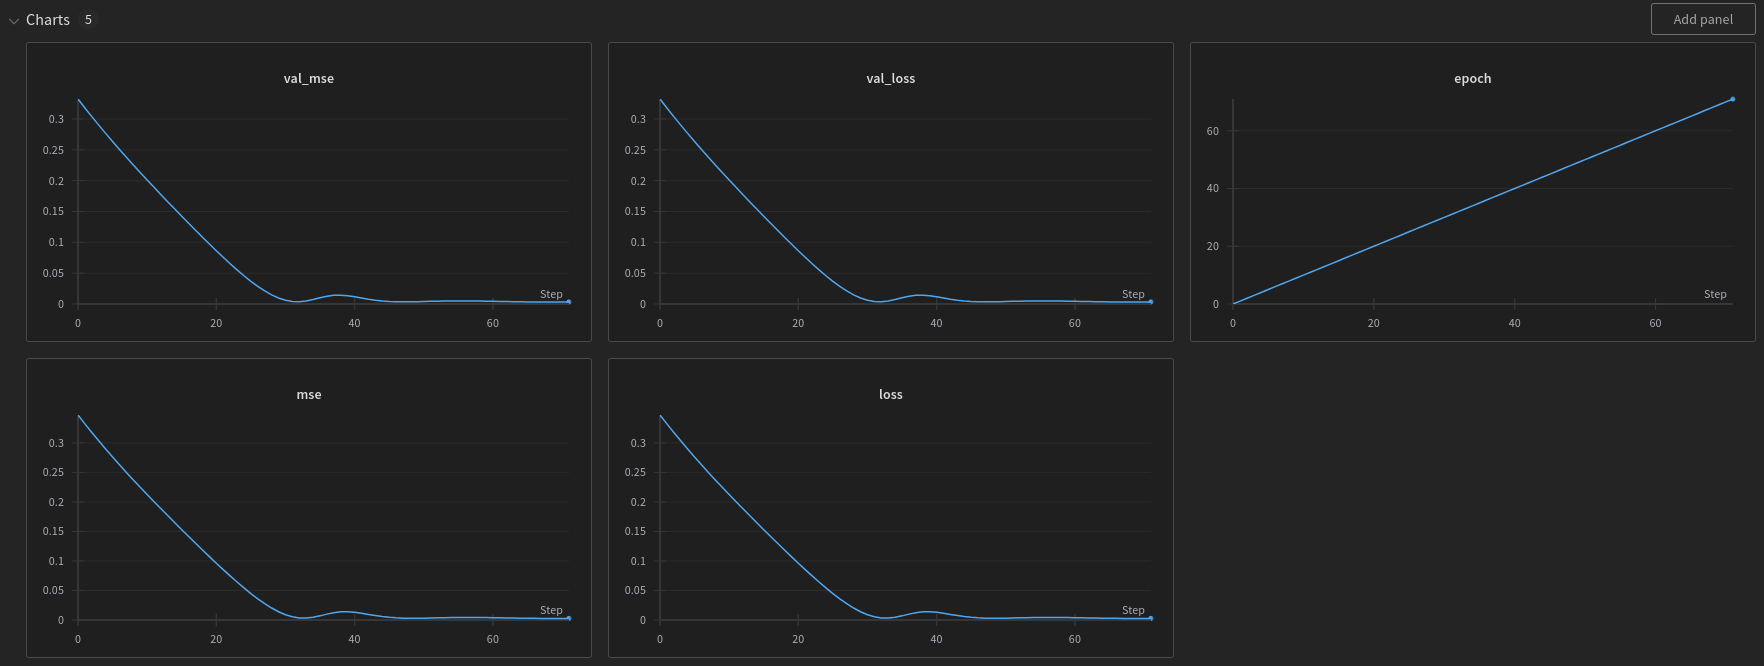
\includegraphics[scale=0.22]{Fig/WyBp1.png}
	\caption{Resultado de entrenamiento del modelo imitador luego de $70$ episodios.}
	\label{fig:Wyb}
\end{figure}	

	\item En la Fig. \ref{fig:errorpen} se muestra una captura de uno de los mensajes correspondientes al error presentado con OpenGL en las pruebas gráficas con $gymnasium$.

\begin{figure}[h]
	\centering
	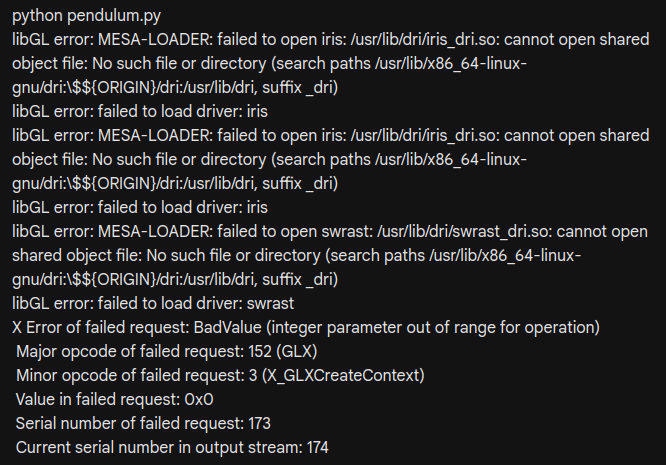
\includegraphics[scale=0.3]{Fig/Errorp1.png}
	\caption{Mensaje de error en prueba de pendulum.py.}
	\label{fig:errorpen}
\end{figure}	

\end{enumerate}









\newpage

\section*{Referencias}
\renewcommand\refname{}
\bibliographystyle{IEEEtran}
\bibliography{references}





\end{document}